\documentclass[NIACPhase1B.tex]{subfiles}

\newcommand{\R}{\mathcal{R}\xspace}
\newcommand{\reals}{\mathbb{R}}
\renewcommand{\S}{\mathcal{S}\xspace}
\newcommand{\cost}{\mathcal{E}\xspace}

\newtheorem{problem}{Problem}

\begin{document}

A cycler is an orbital trajectory where a body encounters two planets on a regular schedule without entering into the orbit of either planet. This periodic encouter without orbiting obviates the need for regular maneuvers, reducing fuel costs and allowing an extremely large vehicle to efficiently travel on this trajectory. Cyclers have been studied for fifty years, with the most famous being the Aldrin Cycler. The Astrotel NIAC examined a mission where a cycler played a central role in the exploration of Mars, and included the Mission Architecture and Model Analysis (MAMA) trade study, which provided a means to chart the roadmap of technologies necessary for the Astrotel concept. 

RHISE expands on this existing work in the cycler mission in two critical ways. One, it \emph{examines} the extensive use of reconfigurability to allow large vehicles to be incrementally constructed over the course of several missions. Two, it \emph{formalizes} the approach taken by the MAMA study, allowing the use of the existing, extensive work in network flow theory and analysis to examine the optimal placement of resources to allow the efficient transfer of humans between Earth and Mars. 

\subsection{Definition}
A cycler is an orbital trajectory where a body encounters two planets on a regular schedule without entering into the orbit of either planet. These trajectories can vary in the frequency with which they encounter the planets, as well as the number and magnitude of maneuvers required to maintain the orbit. Cyclers that require almost no fuel to maintain are known as ``ballistic cyclers'', and because they require little fuel, an extremely large vehicle can travel on the orbit without excessive operating costs. 

\subsection{Background}
Originally introduced by Hollister in the mid-sixties, the most famous of the cycler trajectories is the Aldrin cycler, which is capable of \~6-month traversals between Earth and Mars in one direction, and \~1.5 year traversals in the other. These trajectories can be configured such that the \~6-month traversal is in either the Earth to Mars (Up-) or Mars to Earth (Down-) direction, and so typical cycler missions propose two vehicles, one on each of these orbits, in order to ensure minimal travel time in interplanetary space.

The Astrotel NIAC examined a transportation infrastructure involving cycler vehicles for travel between Earth and Mars. This architecture included several additional support vehicles, including freighters, spaceports, and taxis around multiple other bodies, including the Moon and Phobos. The work culminated in the Mission Architecture and Model Analysis (MAMA) trade study: a full exploration of the range of dependencies which support a such a mission architecture.

The MAMA trade study was designed to allow the identification of critical technologies whose development would help realize the cycler mission. These technologies included cryogenic fuel storage, solar electric and nuclear propulsion, and in-situ resource utilization (ISRU). As a result, the majority of the estimated cost of the mission was in the development of these technologies, with the building blocks of these estimates being high-fidelity analyses of the engineering requirements of each desired capability. 

\subsection{Technical Approach}
A central assumption of the MAMA trade study was the adoption of a relatively traditional approach for the construction of this interplanetary infrastructure, with each of the vehicles reusable but only in the context of their original function. However, the reconfigurability afforded by digital cellular solids can fundamentally change how to approach interplanetary exploration missions. By intelligently selecting orbital trajectories and designing vehicles that are composed of interchangable parts, each mission can lay the groundwork for the next, making subsequent missions more likely to be accomplished.

This novel approach is possible not only because cellular solids can be reconfigured, but also because they allow extensive repairability. That is, a vehicle composed of these parts can recover from failures that would be fatal in a traditionally-designed spacecraft, since parts from another vehicle or part of the ship can be repurposed to replace those that have failed. A similar capability has been shown to provide a sizable reduction in the redundant mass in a typical Mars exploration vehicle's Environmental Control and Life Support System (ECLSS), by using advanced Additive Manufacturing systems to construct spare parts from a generalized feedstock when needed rather than bringing a library of pre-fabricated parts along. 

In order to understand the impact of reconfigurability on the logistics of an interplanetary transport infrastructure, a mission architecture such as the one introduced in the Astrotel NIAC can be extended and formalized as a problem in network flow theory. Network flow theory is a well-explored technique in Operations Research, and has been applied to the optimization of freight transportation networks, air traffic control, and resource distribution. 

Applied to the problem of interplanetary exploration, this approach can allow the efficient survey of the entire problem space of transportation options and infrastructure investments in order to find an optimal solution. In comparison to the MAMA study, it does so by focusing on the formulation of a solution and defining the roadmap of necessary technologies from this solution. This technique will not only be applicable to the Earth-Mars problem but will provide the means of designing other large-scale missions.

\begin{figure*}
\centering
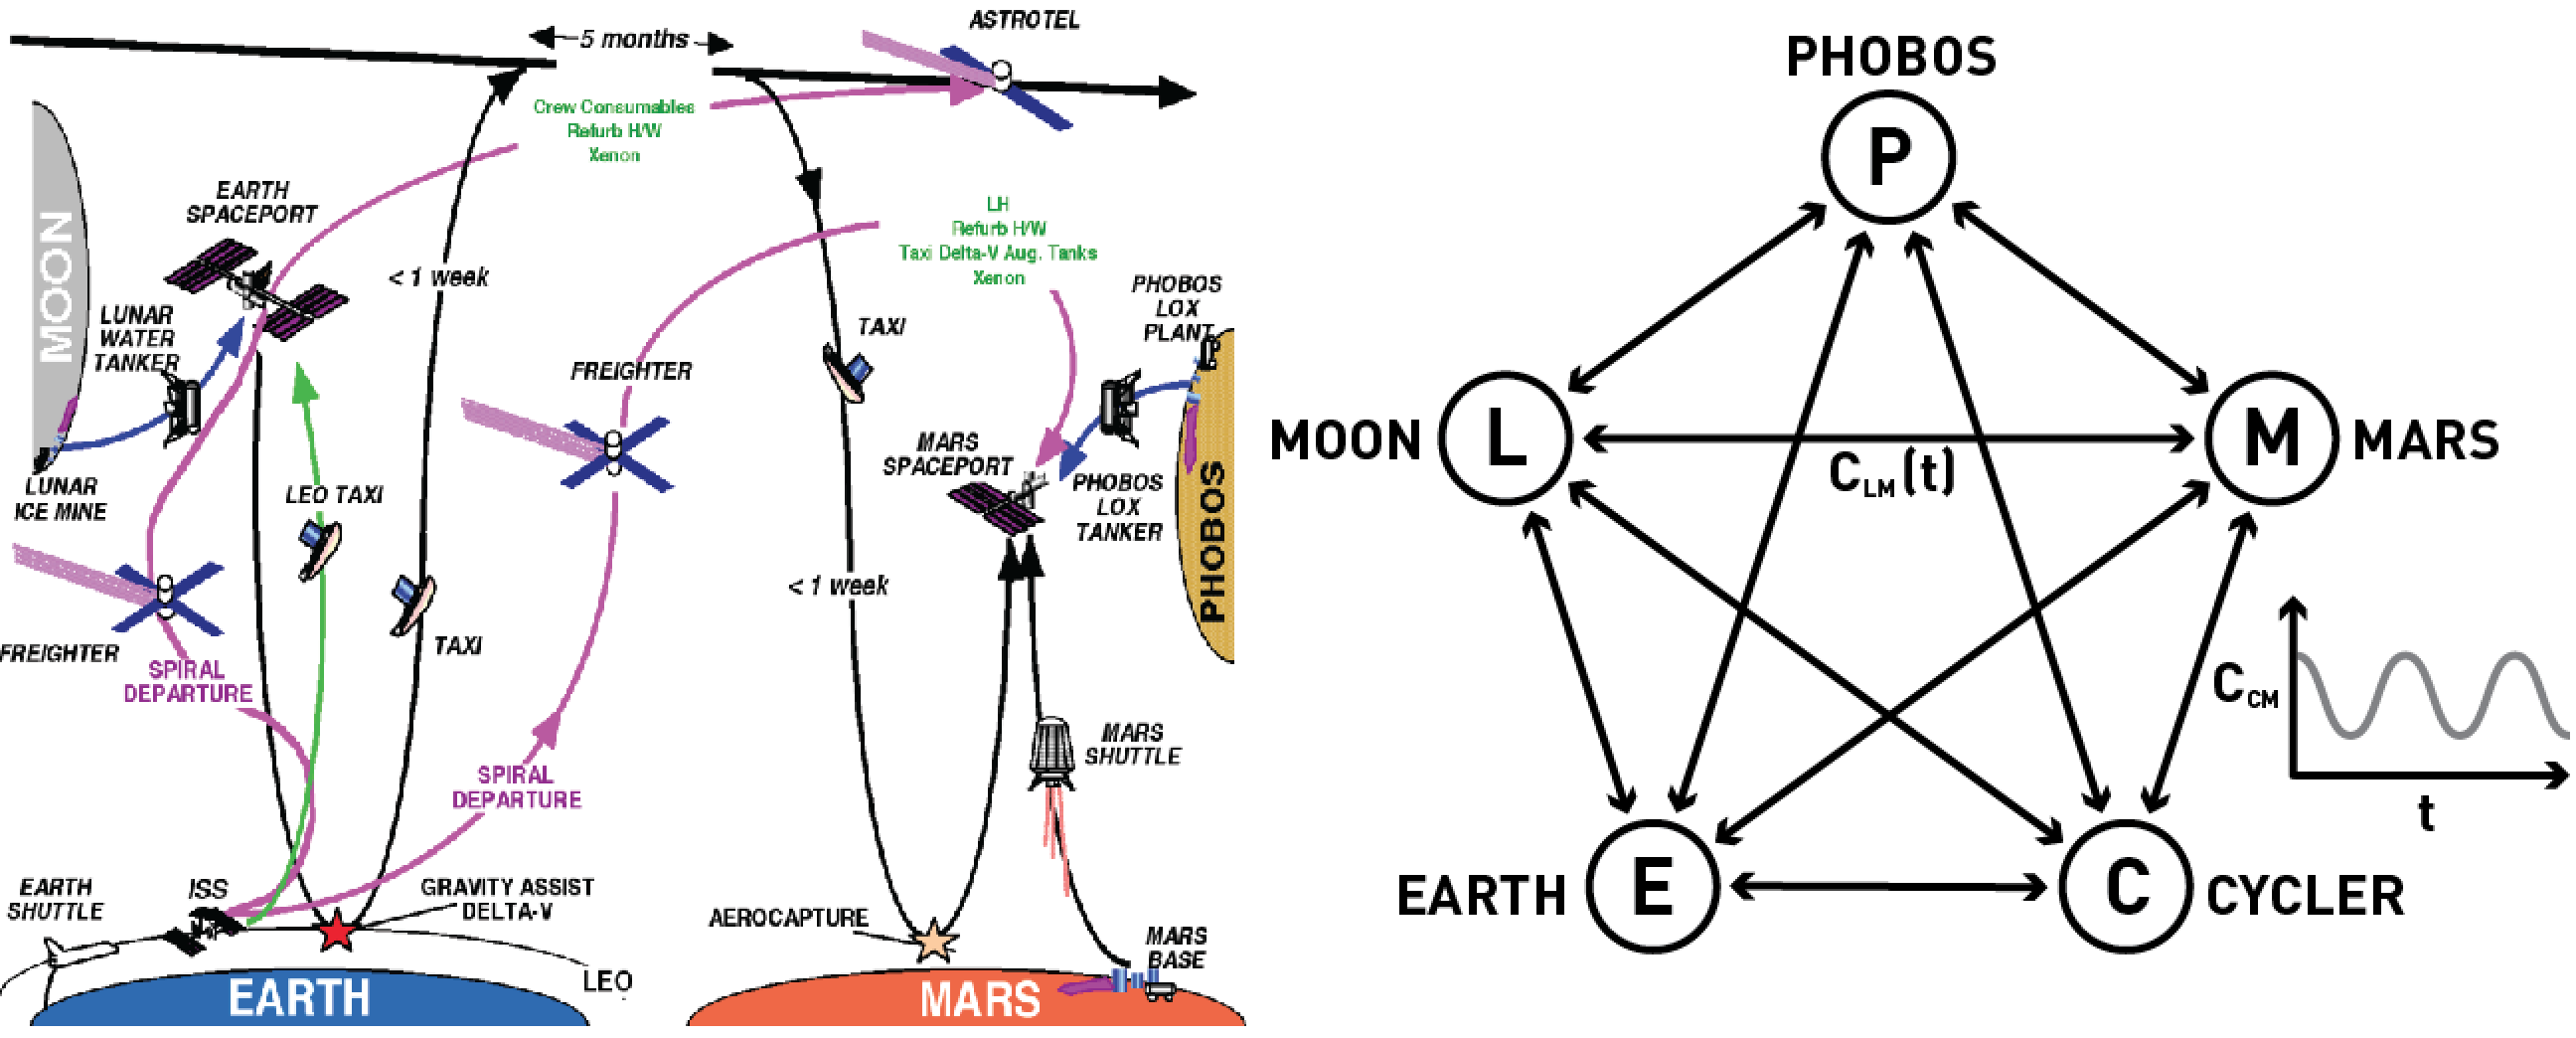
\includegraphics[width=1.0\textwidth]{Media/cycler_opt.png}
\caption{A comparison between previous and the RHISES methods for logistics optimization in a cycler architecture. The left figure is from the Phase 2 report by Nock et. al. and the right figure is an abstraction of the method using network flow theory. Each node in the network represents a destination, with different amounts of various resources ($\rho_1, \rho_2,..., \rho_N$) and connections with cost functions $\zeta^{AB}(t,P)$ that depend on the time $t$ and the resources being sent $P$.}
\end{figure*}

\subsection{Problem statement}

We can formulate the question of designing an optimal cycler architecture as a network flow and scheduling optimization problem in the following way: Consider a network $G=(V,E)$, where $V$ is the set of nodes, and $E$ is the set of directed edges. Each node in $V$ represents a destination point (e.g., Earth, Mars, a cycler). Two nodes $v_1$ and $v_2$ are connected with a directed edge if there is a direct transportation method from $v_1$ to $v_2$.

Consider a set of resource types $\R=\{\rho_1,\rho_2,\dots,\rho_N\}$. These, for example, can include fuel, humans, construction materials, etc. Each node in $V$ can carry some amounts of resources. Moreover, it can produce or spend some resources, depending on the capacity of the node and on the current amounts of resources it is carrying. Denote the rate of change (increase or decrease) of a resource $\rho_i$ at node $v\in V$ at time $t$ as $\sigma^v_i(t,R_v(t)):\reals\times\reals_{\ge 0}^N\rightarrow\reals$, where $R_v=\{r_1,r_2,\dots,r_N\}$ is the amounts of resources being carried by the node at time $t$ (amount $r_j\ge 0$ of resource $\rho_j$ for all $1\le j\le N$). If resource $\rho_i$ is being generated at node $v$, then $\sigma^v_i$ will be positive, and if the resource is being consumed, $\sigma^v_i$ will be negative. Denote the function of change rates of all the resources at node $v$ as $\sigma^v=\{\sigma^v_1,\sigma^v_2,\dots,\sigma^v_N\}$.

To send a payload of resources $P_e=\{p_1,p_2,\dots,p_N\}$ (where $p_j\ge 0$ has type $\rho_j$) along an edge $e\in E$ with the departure time $t$, a certain bulk weight of resources $A_e(t,P_e)=\{a_1,a_2,\dots,a_N\}$ is needed. During the transit some of these resources can get consumed or converted into another type of resource. Denote the amounts of bulk resources that arrive to the destination node as $B_e(t,P_e)=\{b_1,b_2,\dots,b_N\}$. Thus, we can express the rate of change of the resource $\rho_i$ when transferring a given payload $P_e$ along a given edge $e$ as $\zeta^e_i(t,P_e)=b_i(t,P_e)-a_i(t,P_e)$, where $t$ is the departure time. Let $\zeta^e=\{\zeta^e_1,\zeta^e_2,\dots,\zeta^e_N\}$ be the function of change rate for all the resources associated with edge $e$. Moreover, the time it takes to transfer a payload from one node to another can vary. Denote it as $\tau(t,P)$, where $t$ is the the moment of the departure, and $P$ is the payload.

Let $\S=\{(P_i,e_i,t_i)\}$ be a schedule of transfers; it consists of (payload,edge, departure time) tuples. And finally, let $\cost(\S)$ be a cost function of all the transfers in schedule $\S$.

Now we can define the payload transfer problem:
\begin{problem}
Given a network $G=(V,E)$ with functions $\sigma^v_i(t,R_v(t))$ assigned to every node $v\in V$, and functions $A_e(t,P_e)$ and $B_e(t,P_e)$ assigned to every edge $e\in E$, find an optimal schedule $\S^{*}$ of payload transfers in network $G$ that amounts to transferring a set of resources $P=\{p_1,p_2,\dots,p_N\}$ from node $v_1\in V$ to node $v_2\in V$ such that:
\[
\S^{*}=\arg\min\cost(\S)\,.
\]
\end{problem}

\end{document}